% Chapter 5

% variables
\newcommand{\pdirfive}{chapters/plots/chapter5}

\chapter{Future prospects} % Main chapter title
\label{chapter5} % For referencing the chapter elsewhere, use \ref{Chapter1}

The results obtained by the NA64 experiment were already significant to probe a large fraction of the parameter space of the $\umodel$ model, and as shown in the previous chapter many other interesting models, including ALPS, light scalar, and protophobic vector boson are within the reach of this experiment. With the current data, it is already possible to exclude that the dark photon is a viable explanation of the muon anomalous magnetic moment $\ammu$. Most of the parameter space justifying the protophobic vector boson $\DMX$ theorized to justify the anomaly observed in the nuclear spectrum of $^8$Be and $^4$He was also covered by the data collected in the visible mode.

In this chapter, we will explore the prospects of the NA64 experiment, by outlining the main goals remained for the collaboration and by detailing the upgrades that will be performed on the setups. We can summarize the main goals remaining for the NA64 experiment in three items:

\begin{itemize}
\item Cover the region of parameters in the $\dmyplane$ plane most compatible with the relic abundance assuming a freeze-out mechanism taking place in the early universe.
\item Cover the region of parameter space that justifies the $\DM$-anomaly with the existence of a photophobic gauge boson.  
\item Confirm the results of the invisible mode using a $\mu$-beam to probe again the parameter space favoring the currently measured $\ammu$ value.
\end{itemize}

To improve our results, it is straightforward that more data needs to be collected. For the case of the invisible mode, where we are mostly limited by the cross-section of production, improvements in the setup are marginal to increase our signal yield, thus we are mostly limited by the number of EOT accumulated. A value of $5 \times 10^{12}$ was estimated to be a feasible goal to explore the remainder of the parameter space illustrated in Fig.\ref{fig:dm-alpha-excl}. The upgrades of the setup need to address the background that will be encountered for such a large number of EOT, especially the dominant background of electron-hadron interaction upstream of the ECAL.
For the case of the visible mode, on the other hand, the signal yield is dominated by detector efficiency. This means that an improved setup can significantly boost the signal yield, letting us access region of parameter space characterized by a large coupling $\epsilon > 1 \times 10^{-3}$ to finally probe completely the $\DMX$ parameter space.

In Sec.\ref{ch5:sec:mm-upgrades}-\ref{ch5:sec:cal-upgrades} we will present the upgrade for Micromegas detectors and the new ECAL that will be used for the NA64 setup. These upgrades will benefit all setups with a decrease in material budget and larger transverse acceptance. In Sec.\ref{ch5:sec:new-invismode-setup}, we will cover the main upgrades for the invisible mode setup, and give a background estimate for the large data collection expected. In Sec.\ref{ch5:sec:new-vismode-setup}, we will present a new setup optimized to cover the remaining region of $\DMX$ parameter space by taking into consideration the lesson learned by performing a tracker analysis on the 2018 data set. The new setup will also be capable of reconstructing the invariant mass of a particle decaying after the dump, which will permit the measurement of the $\DMX$ to be matched with the one already performed in \cite{Krasznahorkay:2015iga,Krasznahorkay:2019lyl}. Finally, in Sec.\ref{ch5:sec:muon-mode-setup}, we will briefly describe a new concept to use a high-intensity muon beam to probe a novel region of parameter space.
%----------------------------------------------------------------------------------------

\section{Micromegas upgrade}
\label{ch5:sec:mm-upgrades}

\section{Calorimeter upgrade}
\label{ch5:sec:cal-upgrades}

\section{Improvement to the invisible mode setup}
\label{ch5:sec:new-invismode-setup}

The next goal for the NA64 setup is to increase the statistics of the data collected from the current $2.8 \times 10^{11}$ EOT to a total of $5 \times 10^{12}$. This amount will make the experiment sensitive to the interesting region of parameter space compatible with the relic density observed today in the freeze-our scenario and cover a large fraction of the parameter space of pseudo-Dirac and Majorana Dark Matter. Fig.\ref{fig:dm-sens-proj}

\begin{figure}[bht!]
  \centering
  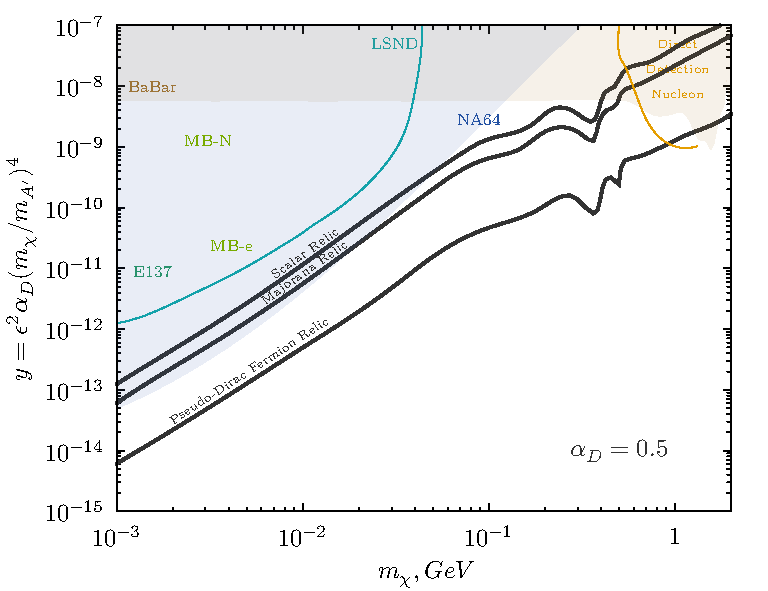
\includegraphics[width=0.45\textwidth]{\pdirfive/tldra-19-2-alpha_0_5.pdf}
  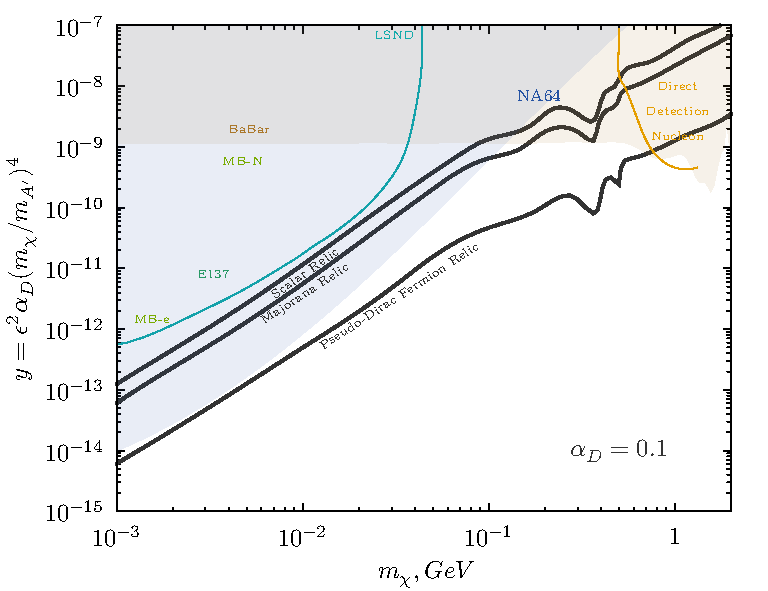
\includegraphics[width=0.45\textwidth]{\pdirfive/tldra-19-2-alpha_0_1.pdf}
  \caption[sensitivity projection for invisible mode 2021]{Limits on the $\dmplane$ plane assuming a number of EOT collected of 5$\times 10^{12}$ by extrapolation of the results obtained using 2016-2018 data set. The parameters are the same used for the calculation presented in Fig.\ref{fig:dm-alpha-excl}. The favored parameters to account for the observed relic DM density for the scalar, pseudo-Dirac and Majorana type of light DM are shown as the lowest solid line.}
  \label{fig:dm-sens-proj}
\end{figure}

Since our signal yield depends exclusively on the cross-section of $\DM$ production, the rate of the signal is expected to be the same. We need to take care of the background expected at this large statistics. We saw in chapter \ref{chapter3} that the dominant contribution comes from electro-nuclear scattering in the beamline before the target. In this section, we will try to study them more in detail and estimate their contribution to a larger sample.

In Fig.\ref{fig:enucl-position} we see the frequency of nuclear interaction for different positions along the beamline after the particle exit the vacuum pipe as predicted from a dedicated MC-simulation. Micromegas detectors are the leading contribution to this background, as a result of their large budget material, which in terms of interaction length is approximate $\lambda_{int} \simeq 1.9 \times 10^{-3}$. It is noticeable however that a factor $\sim 2$ less electronuclear interaction is happening in the first Micromegas of the beamline. This is the result of the smaller material budget of this module, which uses a mylar window instead of a cooper top to close the gas box. Reduction of the material budget of the rest of the module will be an important improvement to suppress this background and has been discussed already in Sec.\ref{ch5:sec:mm-upgrades}. To cover this background, we need to increase the transverse coverage of particles. Naively this can be done by increasing the size of the HCAL, but this solution is rather expensive and would require very large HCAL. Instead, a new detector called VHCAL\footnote{Veto Hadronic Calorimeter} is used for the same purpose. This detector posses the same sandwich structure used for both HCAL and ECAL with a hole in the middle without any material to be aligned with the beam axis. This detector posses lateral size of $50\times50$ \si{\centi\meter\squared}, and is placed upstream the ECAL in front of the vacuum tube exist just after the first tracking detectors as shown in Fig.\ref{fig:vhcal}

\begin{figure}[bth!]
  \centering
  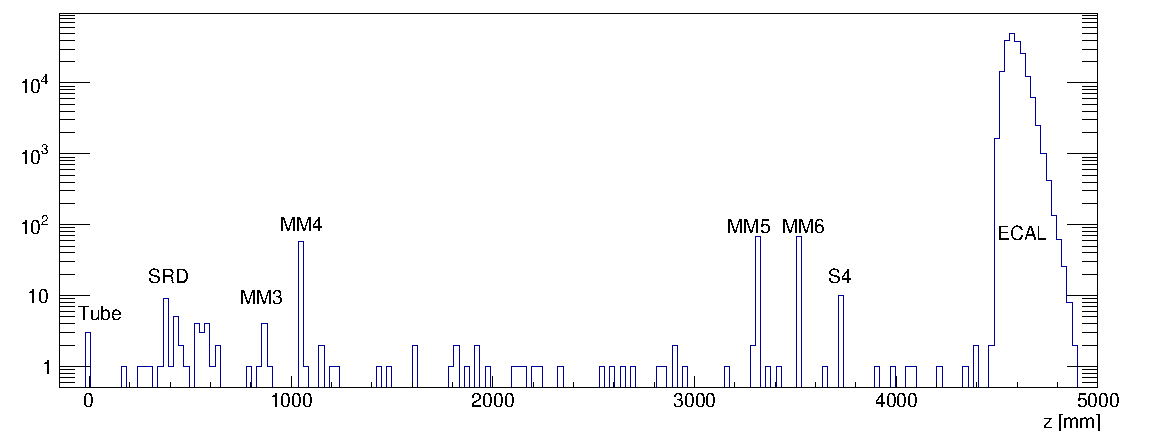
\includegraphics[width=\textwidth]{\pdirfive/enucl-position.pdf}
  \caption[electronuclear interaction position]{Z position of electronuclear interactions between the end of the vacuum tube and the start of the first HCAL. A total of 2.5$\times 10^6$ EOT were simulated for this distribution.}
  \label{fig:enucl-position}
\end{figure}

\begin{figure}[bth!]
  \centering
  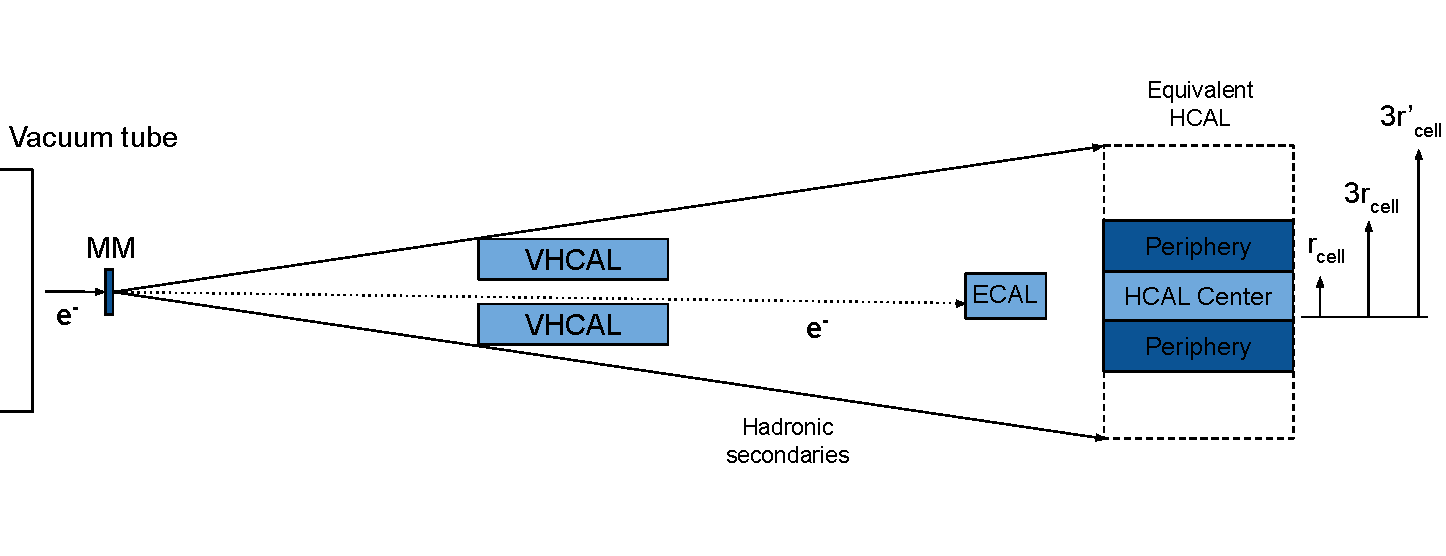
\includegraphics[width=\textwidth]{\pdirfive/VHCAL.pdf}
  \caption[Sketch of VHCAL in invisible mode setup 2021]{Sketch of the VHCAL in the 2021 invisible mode setup. Coverage of large angle particle scattering is shown, together with the equivalent size of the HCAL in this arrangement.}
  \label{fig:vhcal}
\end{figure}

To properly account for this background, we follow the procedure described in \cite{na64-neutrals-study,pdegen-thesis}, which is reviewed here.

First, we divide the $\ehcalplane$ in 10 different zones as depicted in Fig.\ref{fig:enucl-bkg-estimation}. The zones divide the distribution of observed events in several tiles at different distances from the signal region. All the regions labeled with even numbers are events where the energy is conserved and the R-value is closer to the one plotted for region II. In the even within zones labeled with an odd number, on the other hand, some energy is missing from the initial primary electron. The two most relevant are region 7) and 9), which include a part of the signal region. These events have an R distribution closer to the one depicted in region III, with a sharp peak at 1. To further classify the events in these two regions, we can construct a new category based on the value of the R distribution. We define $n_i(r)$ as the number of events in the region $i$ with distance $r$ from the center of the HCAL. This definition let us build a classification of event useful for the background:

\begin{itemize}
\item $n_{5,7}(r=0)$ is the number of events with any energy deposited in the HCAL.
\item $n_{5,7}(r=r_{cell})$ is the number of events with $R=1$, i.e. no energy is deposited in the central cell of the HCAL.
\item $n_{5,7}(r=3r_{cell})$ are the event with no energy deposited in the HCAL, where R is not defined.
\end{itemize}

The final goal is to calculate the probability of an incoming electron primary to produce an event that fall in one of these categories. Which means computing:

\begin{equation}
  \label{eq:enucl-prob}
  p_i = \frac{n_i(r)}{n_{EOT}}
\end{equation}

In practice, the distribution of $n_{i}(r)$ is fitted using an exponential distribution and then integrated in the region $n_i(r>3r_{cell})$ relevant for the background. We are finally ready to estimate the number of events expected for an arbitrary statistic:

\begin{equation}
  \label{eq:exp-bkg-inv-2021}
  n^{bkg}_i \simeq n_{EOT} \times p_i(\lambda \times r)
\end{equation}

In our case, $n_{EOT} = 5 \times 10^{12}$, and $\lambda = r'_{cell}/r_{cell}$ is a scale factor, we define here $r_{cell}$ as the total radius covered in 2018 and $r'_{cell}$ as the equivalent cell radius that will be covered in 2021. Assuming a VHCAL placed at 3 \si{\meter} distance from the ECAL, the coverage would roughly amount to an HCAL with two times its current transverse size, thus $\lambda = 2$. By using our fit for $p_i(r)$ and evaluate it for the zone 7 and 9 relevant for our signal region and $r = 3\lambda = 6$ the maximum region covered by the VHCAL. Our current best estimate for this background is 5$\pm$3 events after taking into account the reduced material budget of the Micromegas \cite{pdegen-thesis}. We illustrate this background extrapolation in Fig.\ref{fig:enucl-bkg-extrapolation} for both region and comparing MC and data, fitted with an exponential distribution.


\begin{figure}[tbh!]
  \centering
  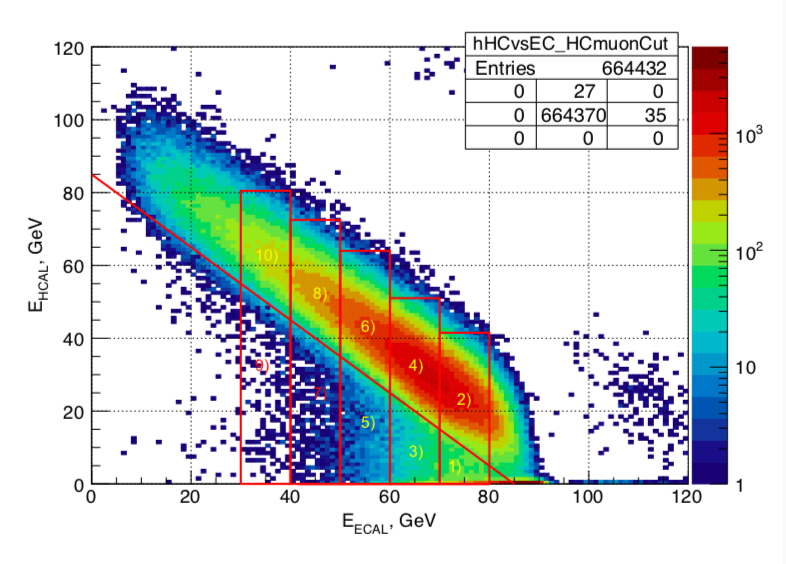
\includegraphics[width=0.45\textwidth]{\pdirthree/zones-no-veto.png}
  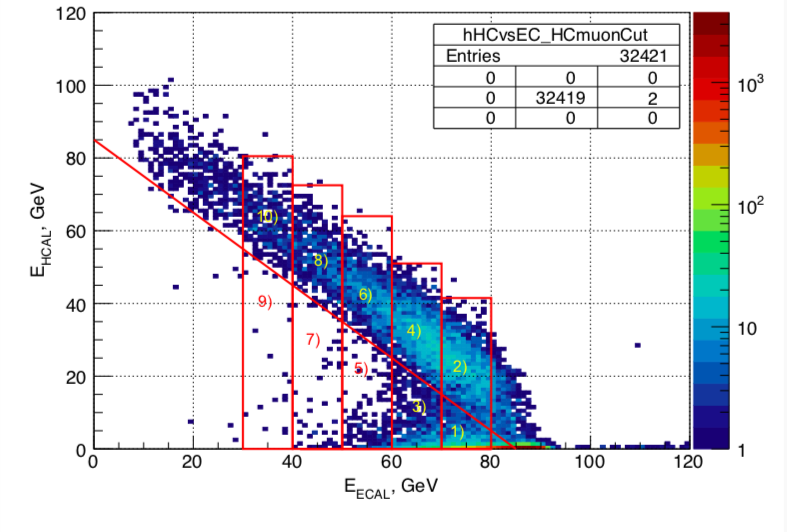
\includegraphics[width=0.45\textwidth]{\pdirthree/zones-veto.png}
  \caption[electronuclear background estimation]{Partioning of the $\ehcalplane$ into ten zones for the background estimation of electronuclear event leaking in the signal box. The left panel shows the control sample of event after clean electron are selected using SRD, tracking, pileup-removal and a hit in the central cell of the ECAL. The right panel shows the same sample after the event with signal in the VETO counter are removed. Adapted from \cite{na64-neutrals-study}.}
  \label{fig:enucl-bkg-estimation}
\end{figure}

\begin{figure}[bth!]
  \centering
  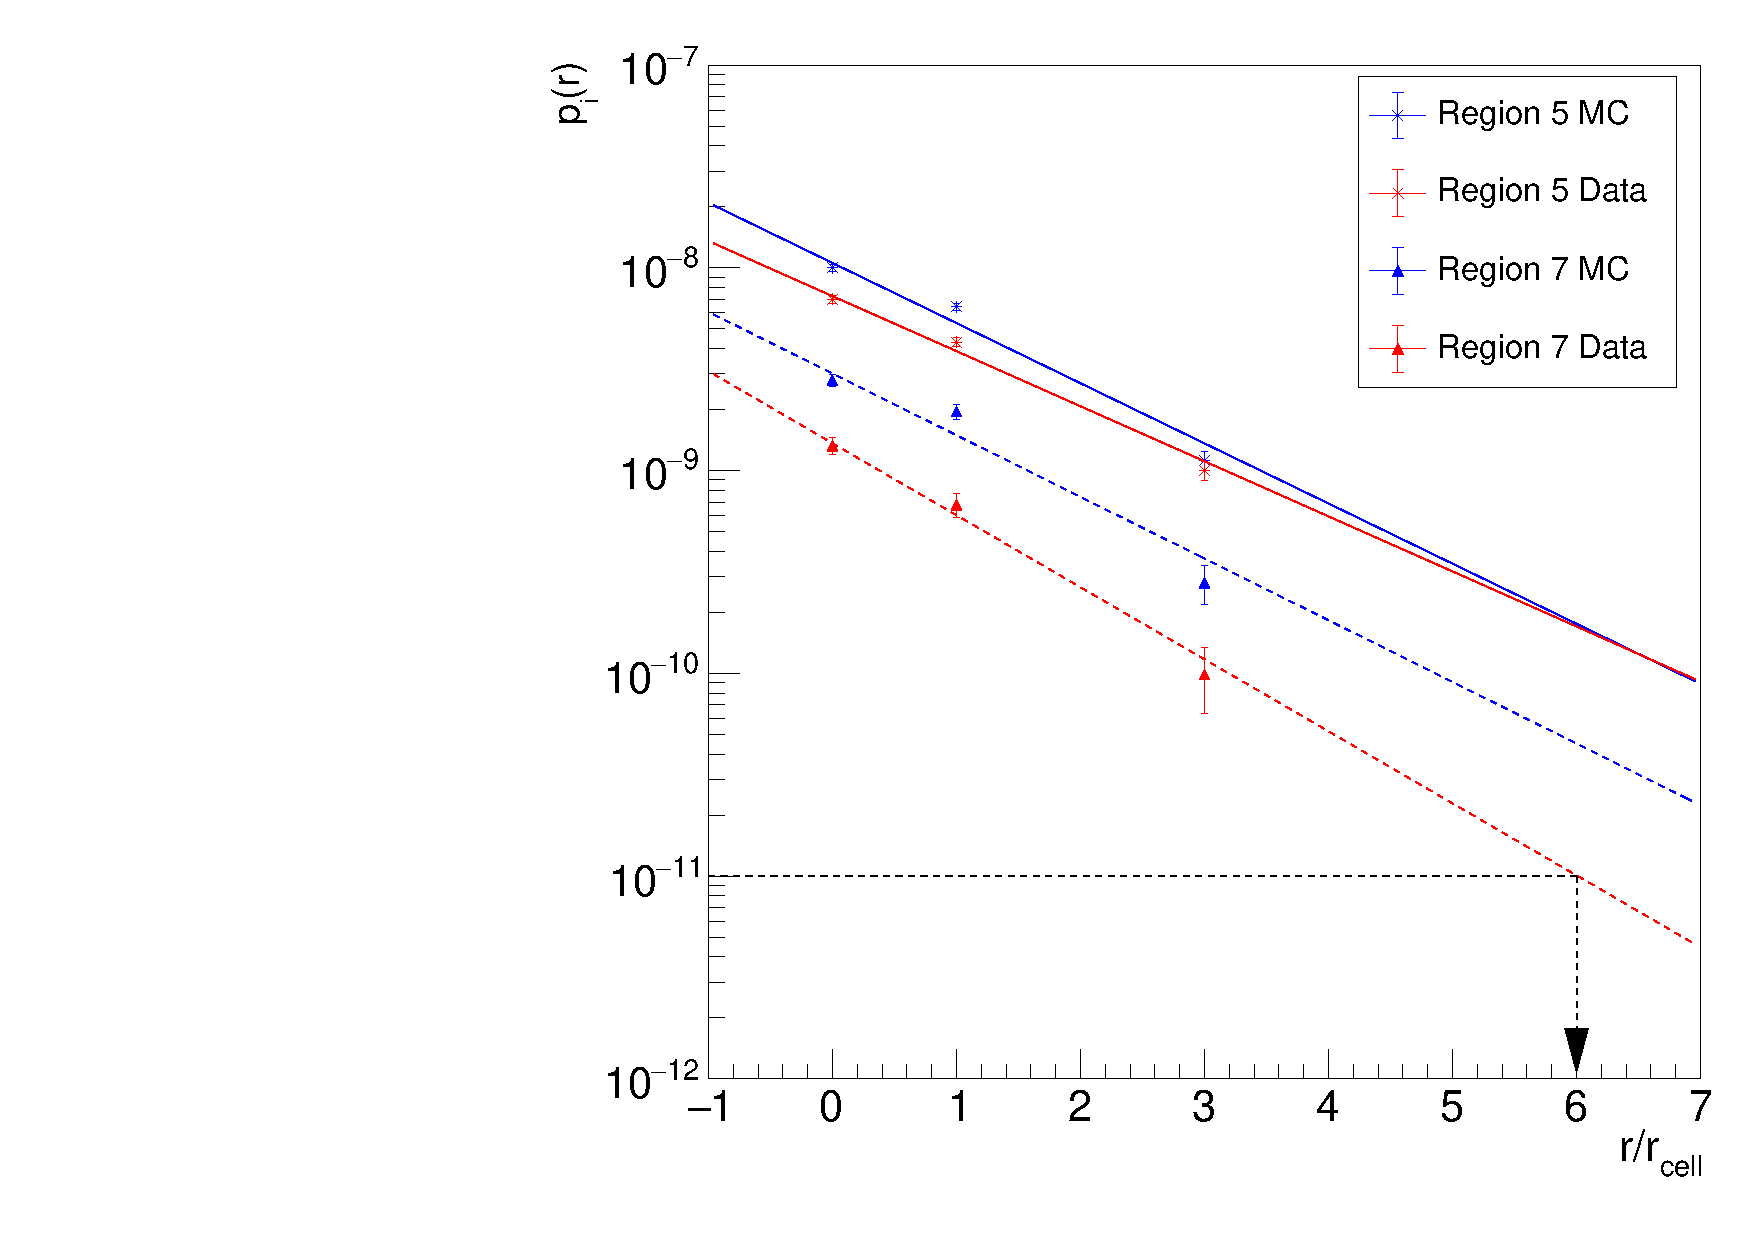
\includegraphics[width=\textwidth]{\pdirfive/pp999-bkg-p.pdf}
  \caption[background extrpolation invisible mode]{Probability of missing energy event as a function of the HCAL transverse size. Extrapolation is performed for both MC and data for region 5 (continuous line) and region 7 (dashed line) as illustrated in Fig.\ref{fig:enucl-bkg-estimation}.}
  \label{fig:enucl-bkg-extrapolation}
\end{figure}

\clearpage

\section{Improvement to the visible mode setup}
\label{ch5:sec:new-vismode-setup}

The main goal of the visible mode data taking in 2021 will be to probe the remaining parameter space that justifies the $\DMX$-anomaly. chapter \ref{chapter1} gives a good description of this model, here we remind that the region in the $\dmplane$ compatible with both the anomaly and the data currently collected by NA64 requires $6.8 \times 10^{-4} < \epsilon < 1.4 \times 10^{-3}$. The mass of $\DMX$ can also be calculated with high precision by fitting the bump in the nuclear spectrum of the anomaly. This procedure currently gives compatible results for the two atoms studied, claiming a mass of 16.70$\pm$0.85 \mev for Beryllium and a mass 16.84$\pm$0.36 \mev for helium. The current setup is unable to probe this particle, as the analysis of the visible mode data has shown. Currently, the main limitation comes from the short decay length of the $\DMX$ and the inability to separate the $\ee$ using trackers. A sufficient setup will need to boost the signal detection efficiency to a level where the $\DMX$ can be probed with a realistic number of EOTs and add a spectrometer able to measure precisely the invariant mass of the $\xdecay$ decay. In summary, to improve the setup we need to address the following items:

\begin{itemize}
\item Increase the probability of the $\DMX$ to exit the dump up to at least 20\%.
\item Increase the distance between the trackers and the decay base of the $\DMX$ to allow the separation of the $\ee$ pair by at least a few mm.
\item Allow the momentum reconstruction of the $\ee$ pair in the $\xdecay$ decay with an accuracy of $\sim$1\%.
\end{itemize}

In the sections that follow, we will explore each of these issues, and give an explanation on they will be solved in the new design of the setup for the 2021 data taking.  Finally, we provide a projection of the EOT and time needed to cover the anomaly completely.

\subsection{Invariant mass reconstruction}
\label{ch5:sec:new-vismode-setup-invmass}

The novel setup proposed for 2021 aims to further improve the background suppression and add the full invariant mass reconstruction for the decay of a very short lived particle generated at the beginning of the dump. In this section, the reconstruction technique is illustrated and the main challenges are outlined. A study based on a full MC simulation of the setup is used to demonstrate the power of the method and its capability of probing the parameter space left to justify the $\DM$ anomaly.

The remained unconstrained parameter space for the coupling $\epsilon$  corresponds to a extremely short-lived $\DM$ with the lifetime $\tau_{\DM} \lesssim 10^{-13}$ s. If we compute the decay length of the $\DM$ we find 
\begin{equation}
L_{\DM} = 28.3 ~{\rm mm}  \Bigl[\frac{E_{\DM}}{100~ \text{\gev}}\Bigr] \Bigl[\frac{17~ \text{MeV}}{m_{\DM}}\Bigr]^2 \Bigl[\frac{10^{-3}}{\epsilon}\Bigr]^2
\label{eqn:length}
\end{equation}
Hence, the energy of the produced $\DM$ has to be $\gtrsim$100 \gev to have the decay length 30 mm comparable to the dump.
Additionally, as $E_{\DM} \gg \mee$, the minimal $\ee$ opening angle and the invariant mass are given by
\begin{equation} 
\angee^{min} \simeq  \frac{2\mee}{E_{\DM}},
\label{eqn:angle}
\end{equation}
\begin{equation}
\mee = [E_{e^+} E_{e^-}]^{1/2} \angee
\label{eqn:imass}
\end{equation}

For an energy $\sim$100 \gev, the average angle is $\sim$0.34 mrad, which is challenging to be measured with precision $\lesssim 10\%$. Instead, we use the short decay length to fix the vertex position of the $\xdecay$ decay and we reconstruct $\angee$ from the separation of the $\ee$ pair in the trackers placed downstream. As the $\DM$ is a short-lived particle, its decay vertex $Z_{\DM}$ is located at the vicinity of the WCAL $Z_{WC}$. This means that $Z_{\DM} \simeq Z_{WC} \ll L_D$ where $L_D=Z_{T1}-Z_{\DM}$ is the distance from the decay vertex and the first tracking detector (see Fig.\ref{fig:imass_sketch}). Since $L_D \simeq Z_{T1} - Z_{WC}$, the opening angle $\angee$ can be evaluated as 
\begin{equation}
\angee \simeq \arctan{\frac{ L_{\ee}}{L_D}}
\label{angle-est}
\end{equation}
where $L_{\ee}$ is the distance of the $\ee$ pair in the T1 plane. Using error propagation, we can estimate the uncertainty on the angle:

\begin{equation}
  \sigma^2_{\angee} \simeq (\sigma_{L_{\ee}}  / L_D)^2 + (\sigma_{L_D} / L_D)^2(L_{\ee} / L_D)^2,
  \label{eqn:thetaerr}
\end{equation}

where $\sigma_{L_{\ee}}$ is the hit resolution of the tracker and $\sigma_{L_D}$ is the error of the decay base. In our conditions, the second term is negligible due to the high precision of our tracking detectors and the large distance between them and the target. The formula above shows that a tube of $\sim$10 m is sufficient to reconstruct the invariant mass with a precision $\lesssim$10\%. However, this estimate is flawed by the fact that hit resolution worsens as the two hits are closer.

\begin{figure}[bth!]
  \centering
  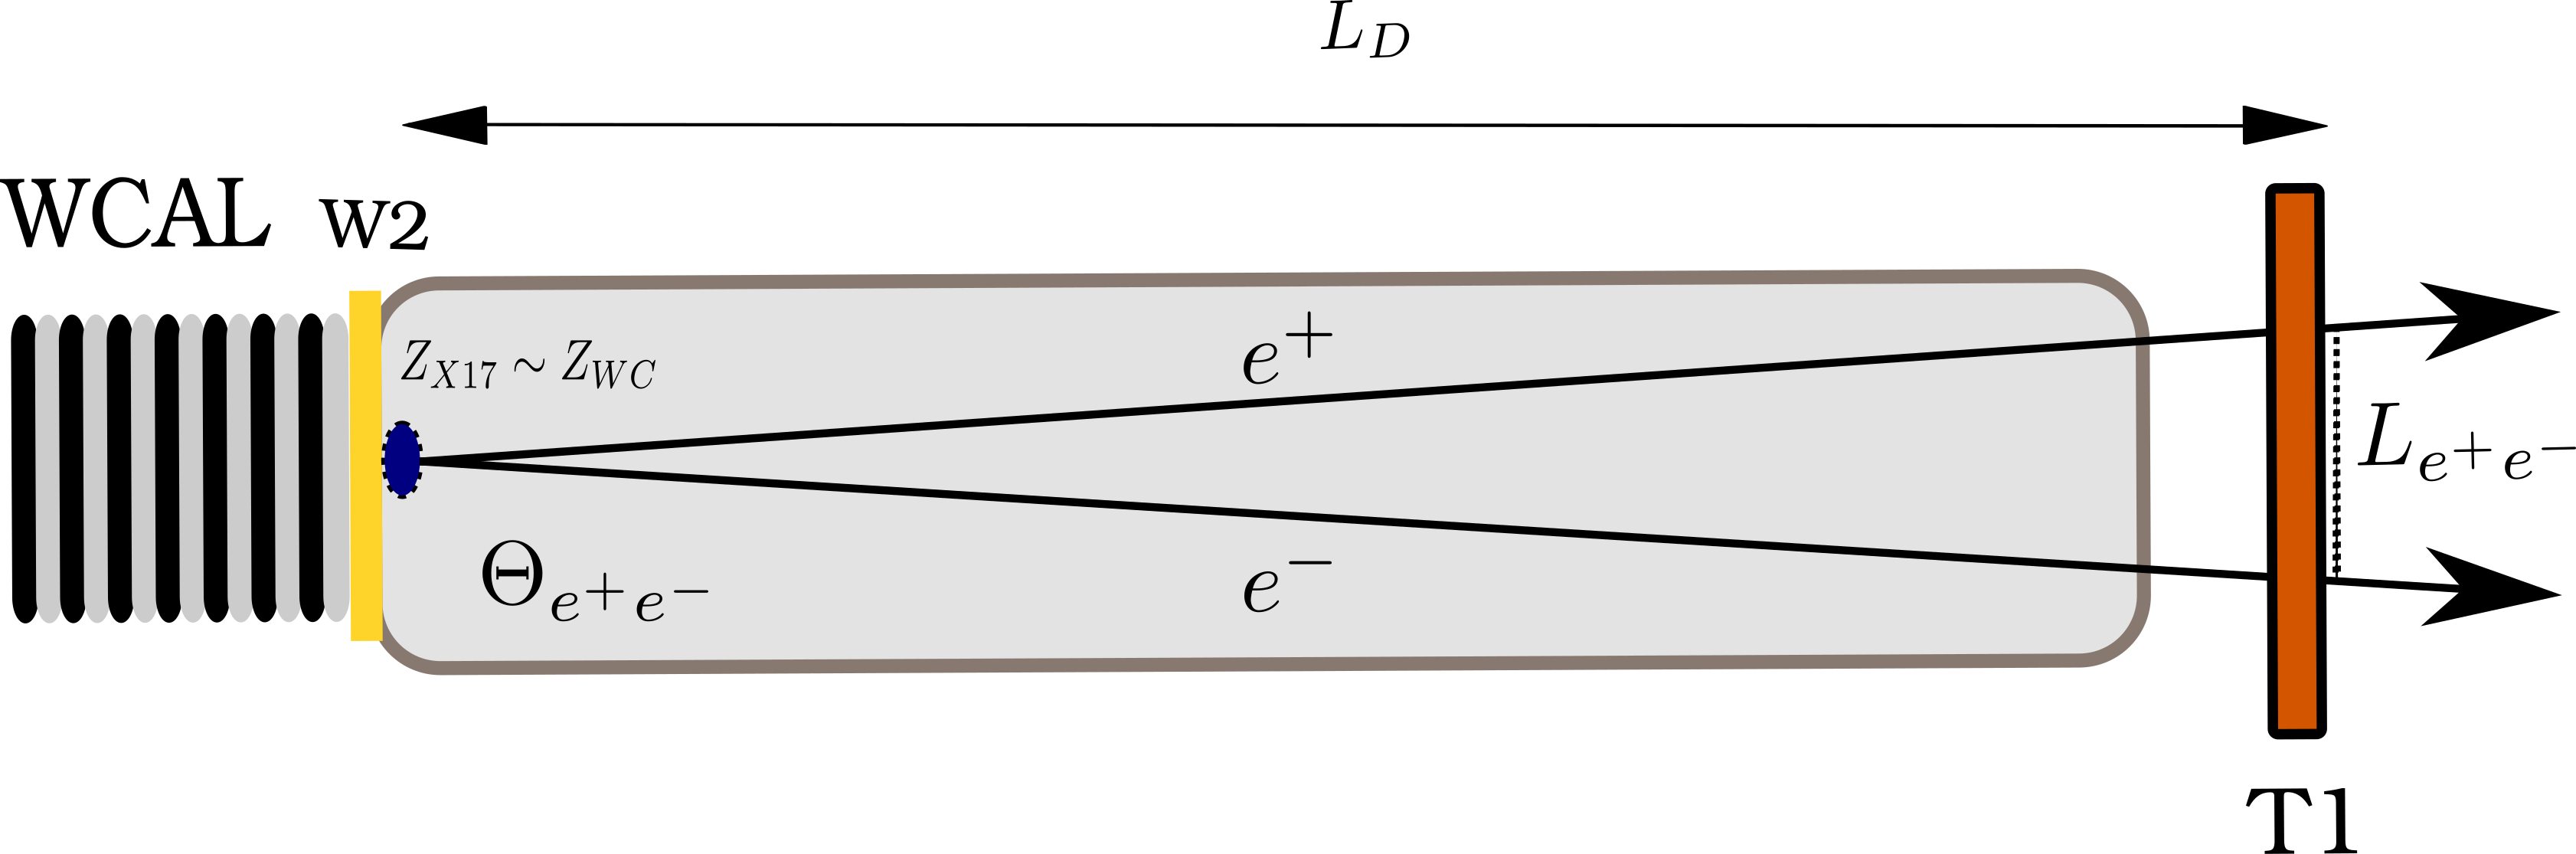
\includegraphics[width=\textwidth]{\pdirfive/imass_sketch.png}
  \caption[Invariant mass reconstruction sketch]{Sketch of the $\DM$ decay in the proposed setup along the beam axis.}
  \label{fig:imass_sketch}
\end{figure}


This problem has been studied using both fitting procedures and neural networks to reconstruct the original hit position from two overlapped clusters. The data recorded with a gas detector during past NA64 runs were used to build a set of different possible topologies. A new set to test different algorithms was then created by mixing these clusters randomly. An example of such a study, where the two clusters are separated using a global fit of two Gaussian is presented in Sec.\ref{ch5:sec:separ-hit-micr}. Both procedures agree that the hit resolution worsens to a maximum of 200 $\mu$m when the separation is lower than 1.5 mm. No significant worsening in the resolution is observed when the distance between hits exceeds $\sim$2 mm. In the proposed setup, a distance of 18 m is used between the dump and the first tracker, getting an average separation of 5.5 mm (Fig.\ref{fig:dm_dist1}). As our data-driven studies have shown, the hits should be well separated in each signal event, granting a hit resolution of 80 $\mu m$ for the $\ee$ pair.

\begin{figure}[tbh!]
  \centering
  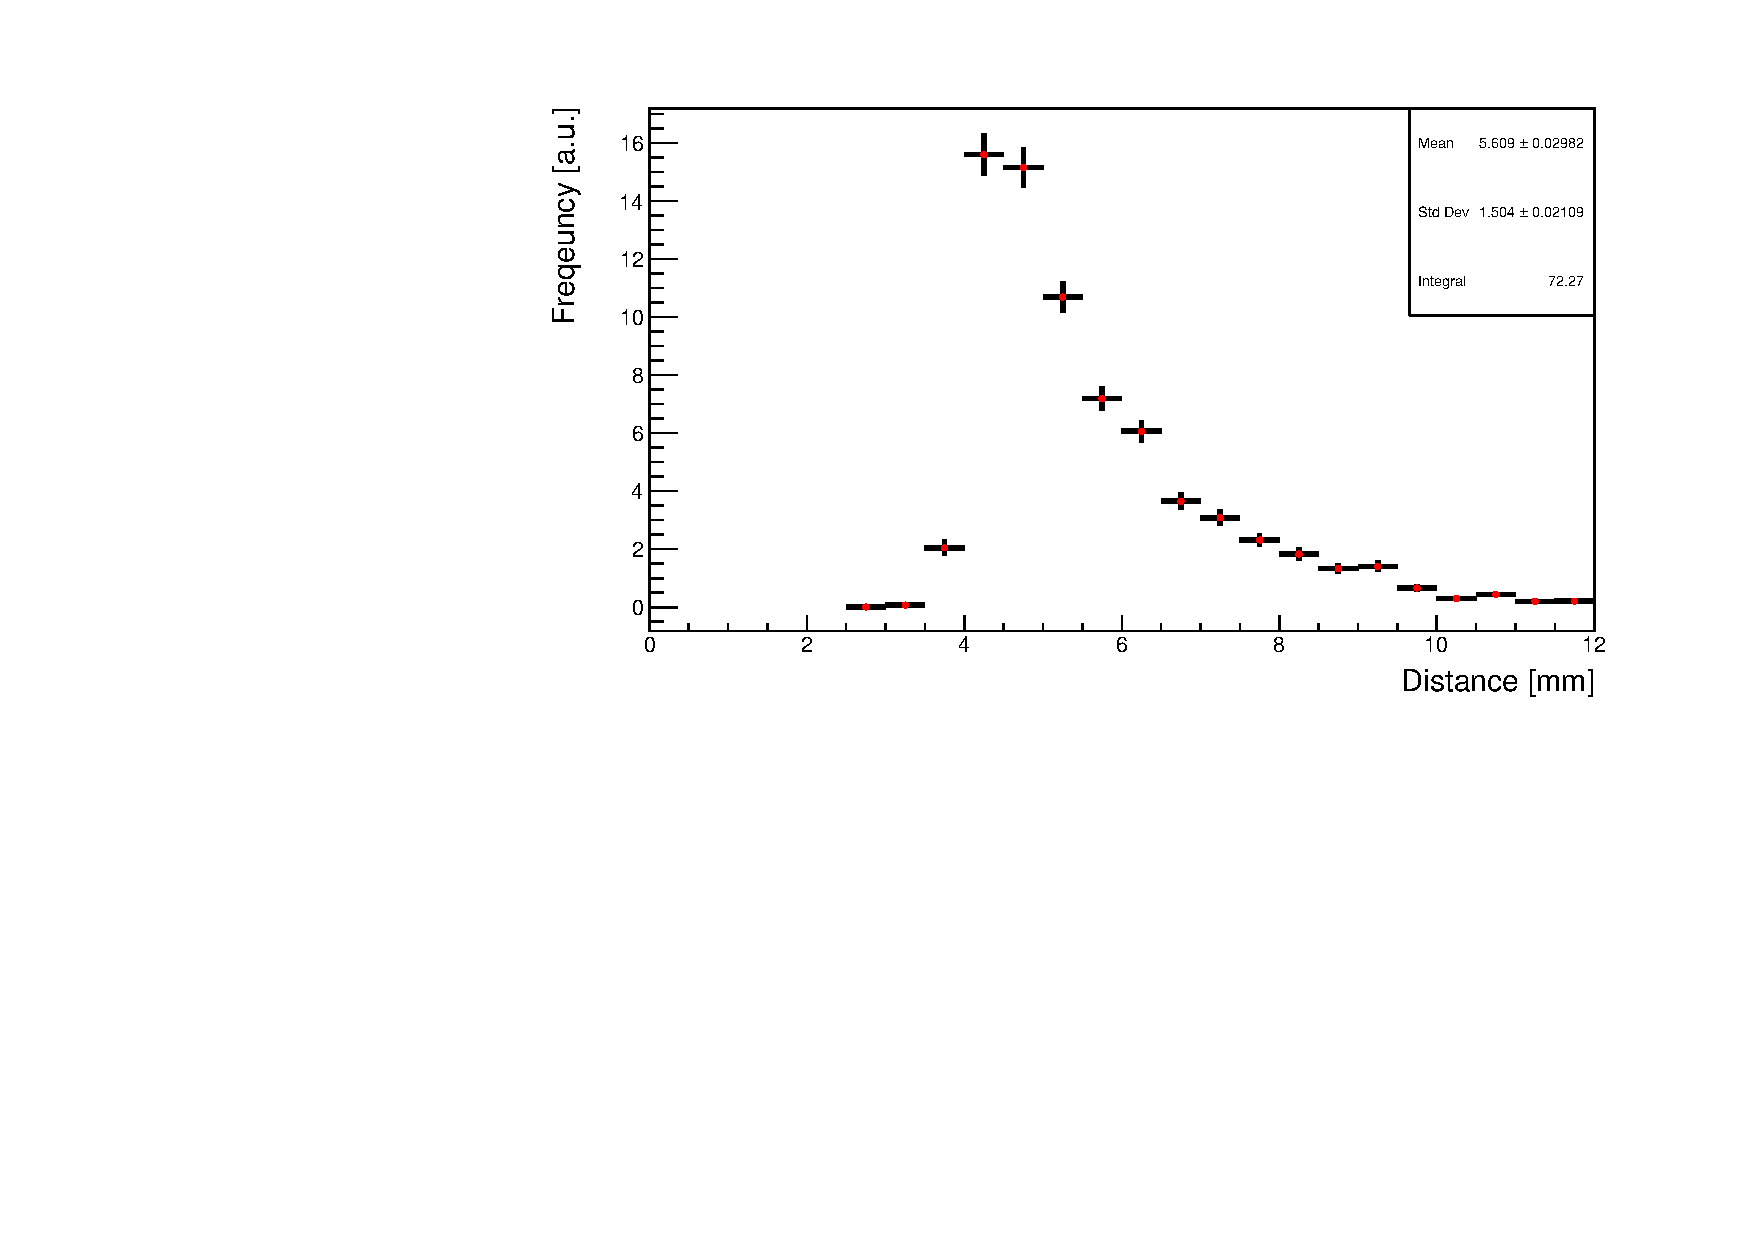
\includegraphics[width=\textwidth]{\pdirfive/DM-dist.pdf}
  \caption[Distance of the decay products of X17 in the 2021 setup]{Distance between decay products of an $\DM$ decay outside the dump at a distance of 18 m from the decay vertex.}
  \label{fig:dm_dist1}
\end{figure}

To complete the invariant mass reconstruction one needs to know with high precision the momentum of the decay products in a signal-like event. Two independent measurements are used for this purpose. The first one is the momentum reconstruction of the two tracks after passing through a magnetic field. The second one is the measurement of the same two tracks energy in two well-separated em-showers in the ECAL downstream. A dipole magnet bends the two tracks and separate them to reconstruct their energy with a precision of 10\%$/\sqrt{\gev}$ in the ECAL. To achieve this purpose a separation of at least two ECAL cells ($\sim 8$ cm) is needed.

The setup proposed uses an 18 m vacuum tube kept at a pressure of 8$\times 10^{-4}$ mbar. Two GEM trackers \cite{gem} are placed at a distance of 0.1 m and 2.1 m respectively from the end of the tube. A magnet is placed immediately after the second GEM to separate the two tracks that are detected by a set of GEM trackers placed at 0.3 m and 1.3 m from the end of the magnet. Finally at a 3.4 m distance from the end of the magnet the ECAL is used to measure the energy of the incoming particles. A sketch of the setup can be seen in Fig.\ref{fig:setup-2021}.

\begin{figure}[tbh!]
  \centering
  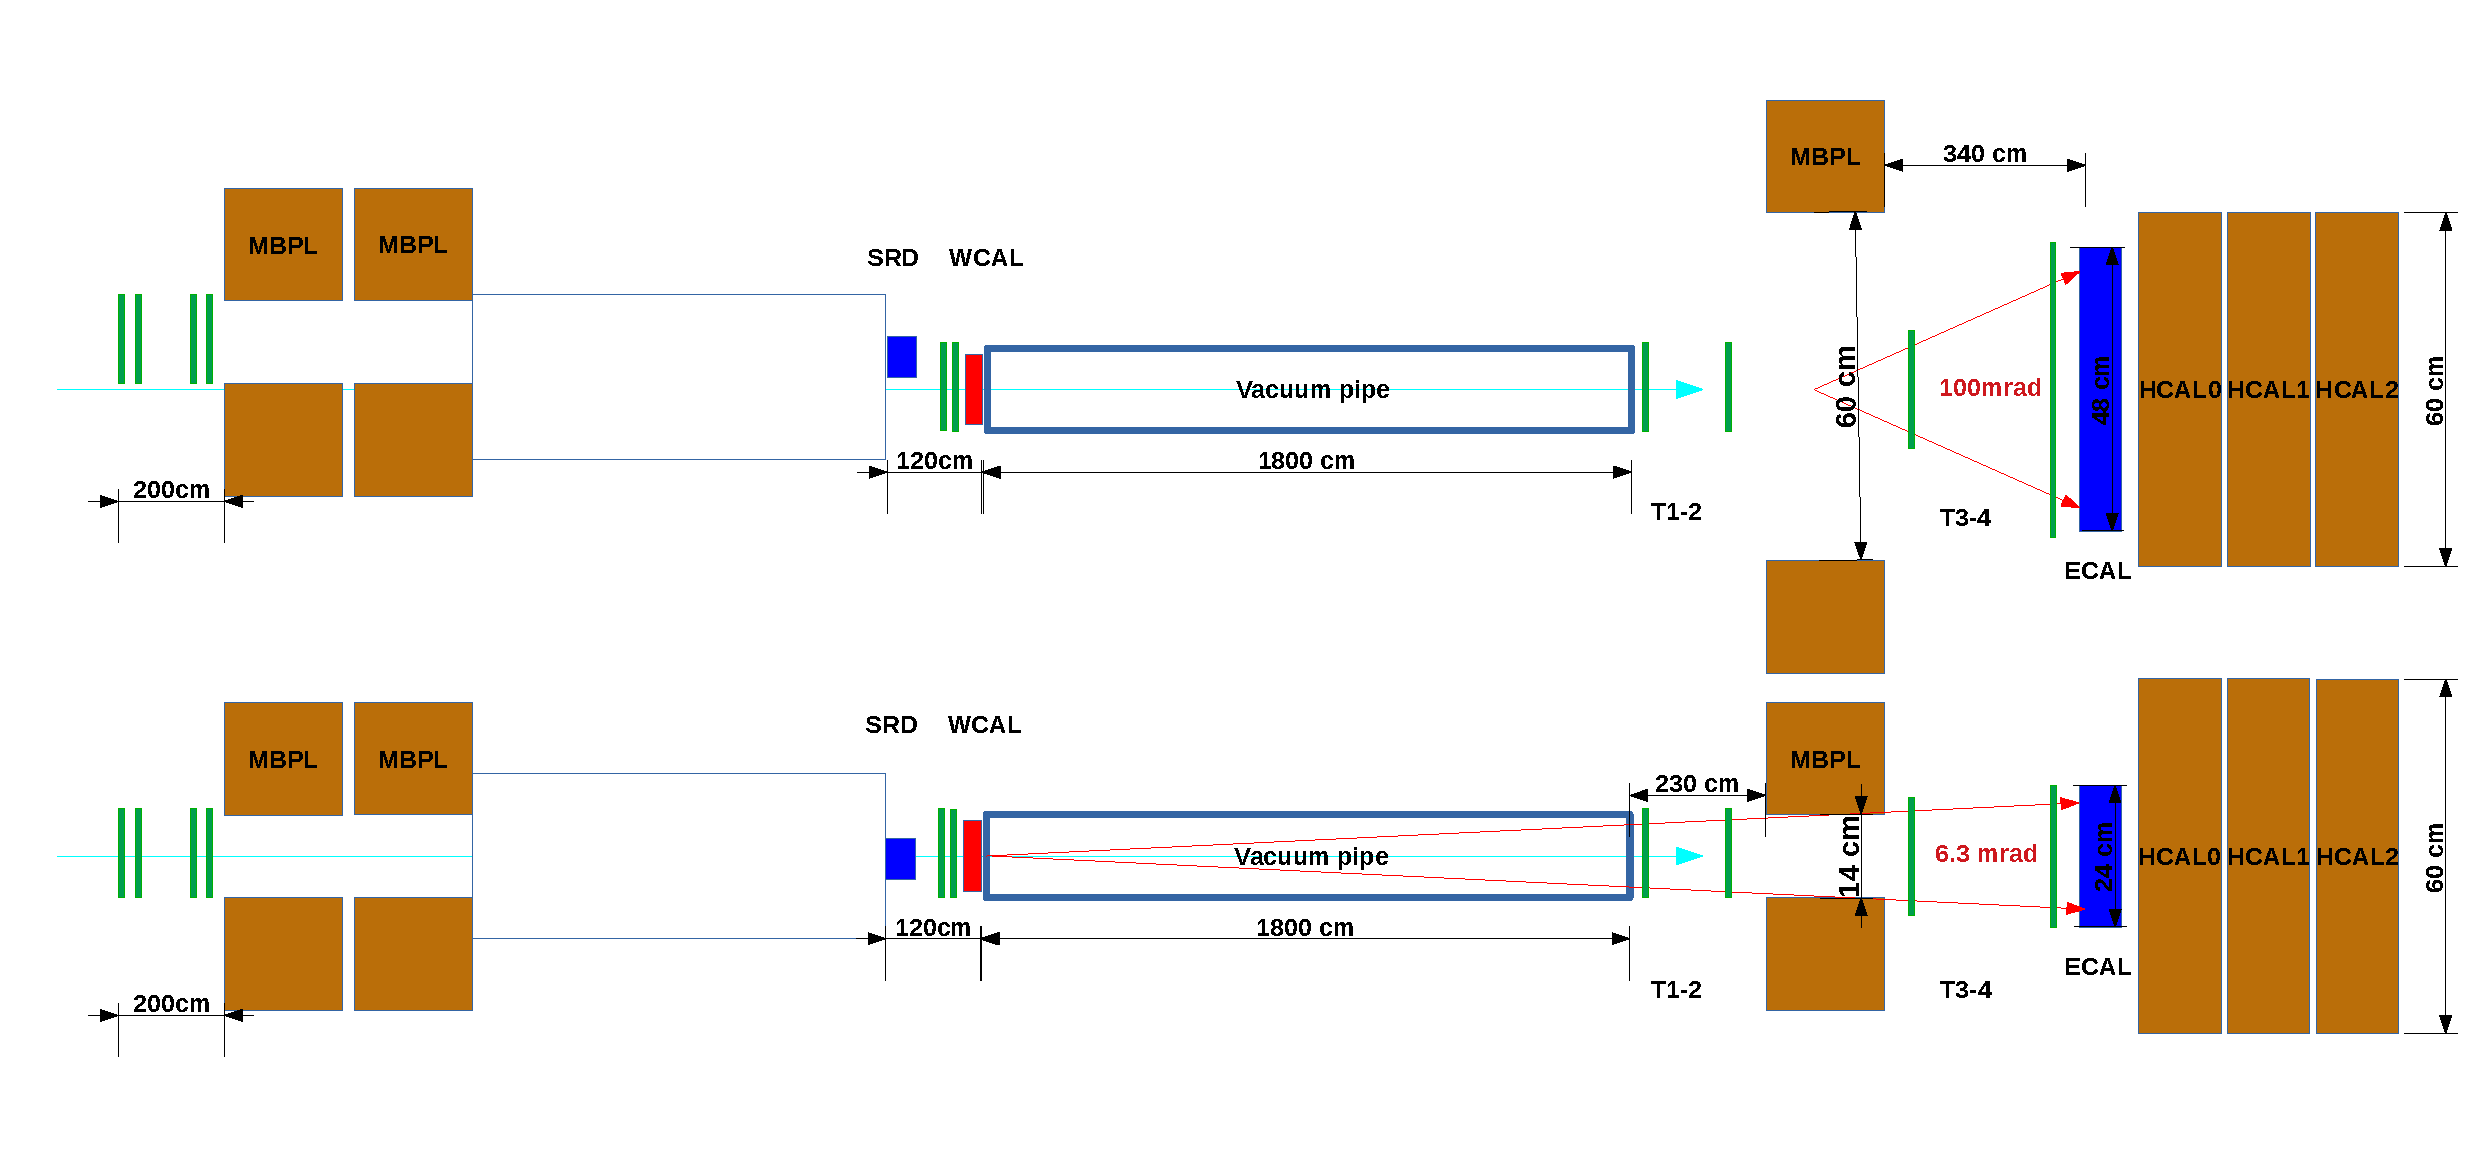
\includegraphics[scale=0.33]{\pdirfive/setup-2021.pdf}
  \caption[2021 setup]{Sketch of the setup proposed for the 2021 visible mode of NA64. Top view and side view are shown in the top and bottom pictures respectively.}
  \label{fig:setup-2021}
\end{figure}

The invariant mass is reconstructed with a precision of $\sim$2\% (Fig.\ref{fig:imassreco}). The fit is performed using the sum of two Gaussian functions with a shared mean corresponding to the best estimate of the invariant mass. Furthermore, 90\% of all events are reconstructed with an error smaller than 10\%. This reconstruction was performed using a MC simulation where all detectors budget was reproduced precisely to estimate the impact of the multiple scattering. This is detailed in Sec.\ref{ch5:sec:mm-scattering}.


\begin{figure}[tbh!]
  \centering
  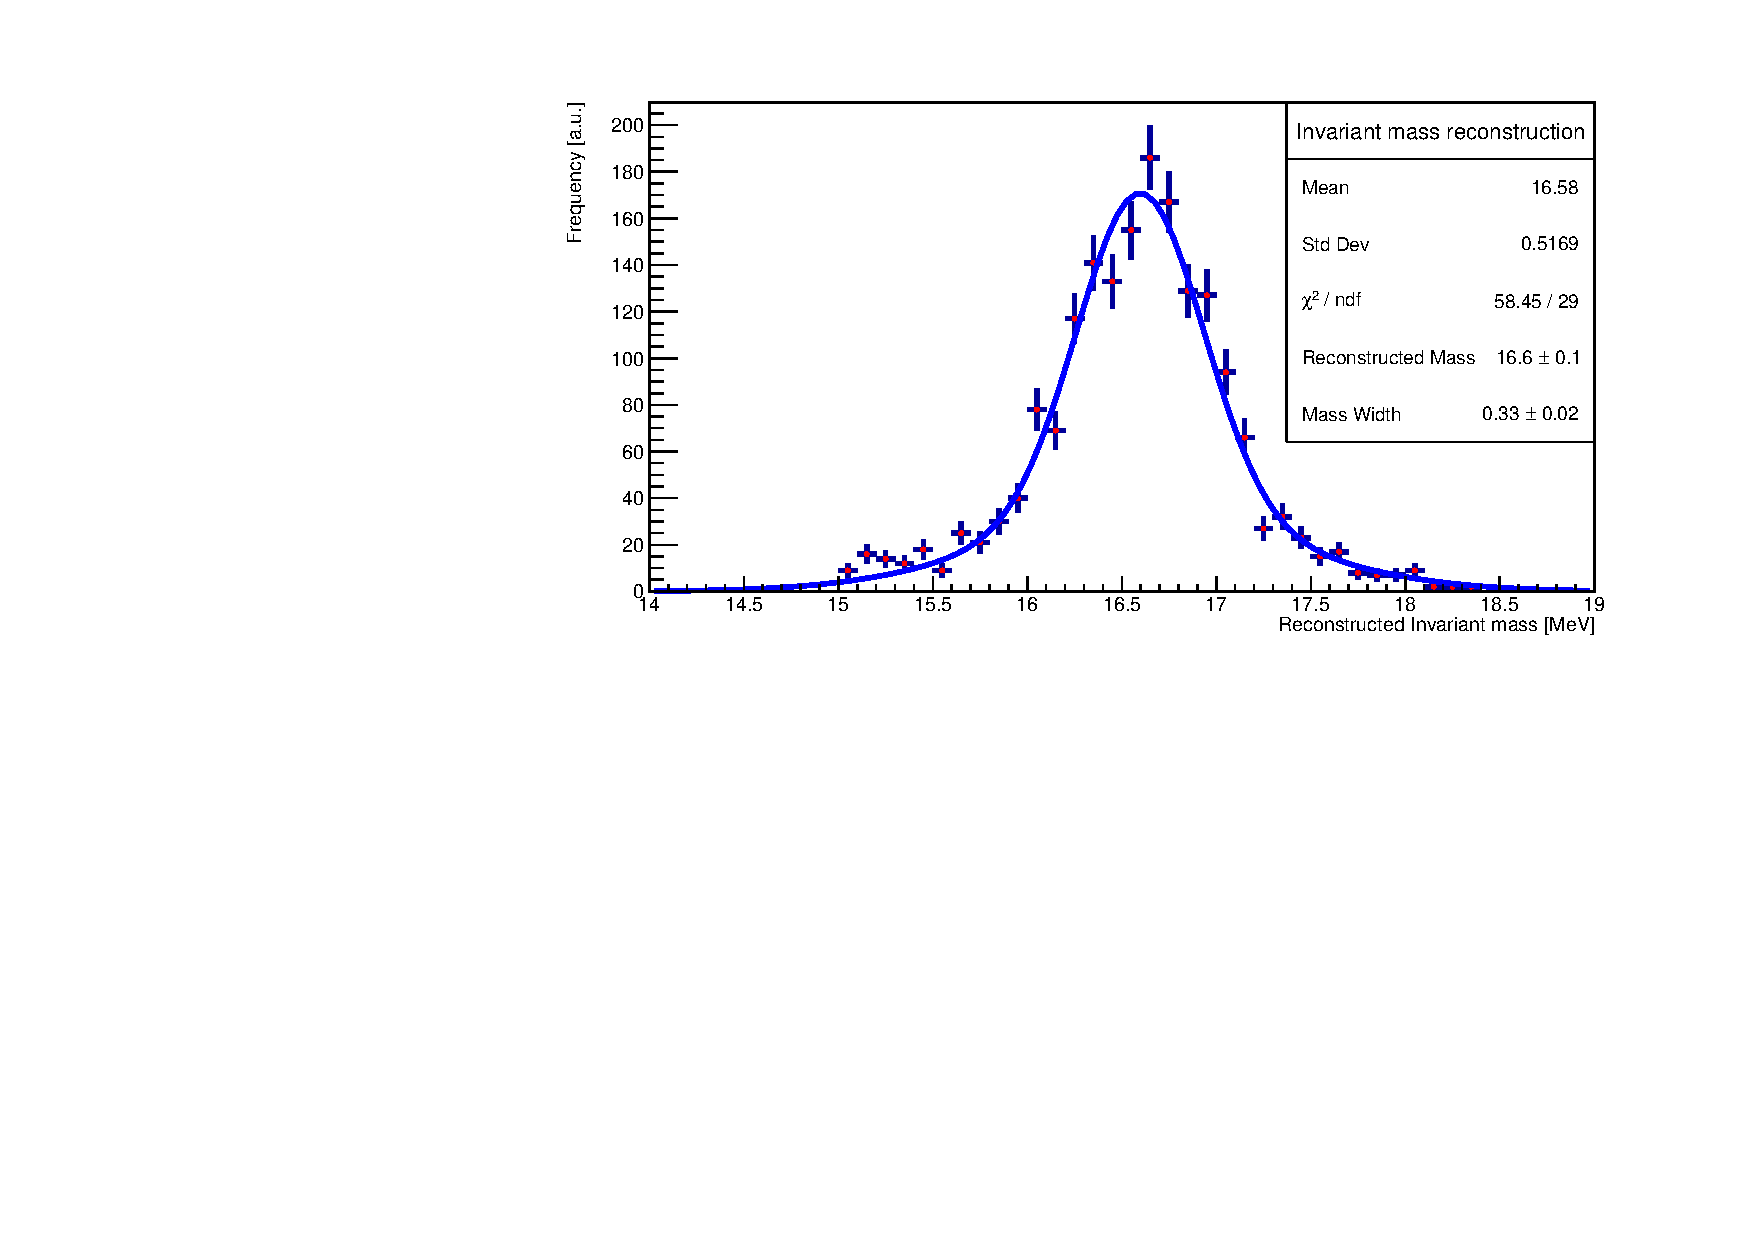
\includegraphics[scale=.8]{\pdirfive/invariant-mass-reco-allcuts.pdf}
  \caption[Invariant mass reconstruction in 2021 setup]{Reconstructed invariant mass of $\DM$ in 2021 setup after weighting each event by its possibility to decay outside the dump. 90\% of all events considered are reconstructed with 10\% precision. A fit performed with the sum of two Gaussian with same mean is shown as a blue line. The simulation was performed using a $\DM$ with a mass of 16.7 MeV and $\epsilon = 1.4\times10^{-3}$.}
    \label{fig:imassreco}
  \end{figure}

\subsubsection{Multiple scattering effects on invariant mass reconstruction}
\label{ch5:sec:mm-scattering}

An additional source of error is caused by the multiple scattering experienced by the $\ee$ pair produced from the $\DM$ decay. As the decay takes place immediately after the dump, the multiple scattering experienced originates from:

\begin{itemize}
\item The air pocket between the end of the WCAL and the beginning of the vacuum tube.
\item The two Mylar windows used to seal the vacuum tube.
\item 18 m of low pressure air inside the tube.
\item The air pocket between the tube and the trackers used to measure the distance of the two decay products.
\end{itemize}

Additionally, one has to consider that the thickness of W2 placed after the WCAL can also have an impact on the multiple scattering. This effect is however suppressed since most of the $\DM$ where the decay vertex is inside the W2 are normally removed from the analysis by the requirement of small energy deposit in this active area. The thickness of this counter was minimized to 3 mm from the 6 mm used previously. This reduces the contribution of multiple scattering and at the same time increase the $\DM$ detection efficiency since the dump length is further reduced.

Therefore to ensure a small impact on the invariant mass reconstruction. The vacuum tube is placed attached to the WCAL aluminium box to minimize the air pocket down to $\sim$1 mm. Moreover a thin 175 $\mu$m Mylar window is used to seal the vacuum tube which is then kept at a pressure of 8$\times 10^{-4}$ mbar. The first detector is placed immediately attached to the vacuum tube to reduce the air interaction to a minimum. The second Micromegas tracker is placed at 2 m distance from the first one to compromise between angle and momentum resolution. All the materials were added in the MC simulation of the setup and their effects were studied in detail. The conclusion of this study is that the multiple scattering has a small impact on the precision of the reconstructed invariant mass, the degradation observed compared to a scenario where only perfect vacuum is present between the end of the WCAL and the first tracker is $\sim$0.1\%. The contributions on the invariant mass width, including limited position resolution and momentum reconstruction, are summarized in Table \ref{tab:imass-width}.

\begin{center}
  \begin{table}[bth!]
    \centering
    \begin{tabular}{|l|r|}
      \hline
      Error source & Mass width [MeV]\\
      \hline
      setup in vacuum & 0.11\\
      trackers hit resolution & 0.29\\
      vacuum window + air & 0.31\\
      momentum reconstruction & 0.33\\
      \hline
    \end{tabular}
    \caption[Error budget for the invariant mass in 2021 setup]{Width of the invariant mass after different error contributions are added cumulatively. In the first entry, all the space in the decay volume is substituted by perfect vacuum, the only material left is the one of the trackers and the W2. In the second entry, a 80 $\mu$m hit resolution is added to the trackers. In the third entry, the vacuum is substituted by the realistic setup shown in Fig.\ref{fig:setup-2021}. Finally, the last entry add the effect of the momentum reconstruction. The invariant mass distribution with all effects considered is presented in Fig.\ref{fig:imassreco}.}
    \label{tab:imass-width}    
  \end{table}
\end{center}

\subsubsection{Hit separation in gas tracking detectors}
\label{ch5:sec:separ-hit-micr}

The NA64 experiment uses gas tracking detectors to reconstruct the incoming momentum of the electrons and reconstruct tracks in the decay volume. A set of 8 XY-multiplexed Micromegas and 4 GEM modules were employed in the invisible and visible mode setup for this purpose. As introduced in Sec.\ref{ch2:sec:vismode}, one of the main challenges of the novel setup design will be to separate two tracks at low distance in order to reconstruct the angle of the two-body decay.

A set of clusters was extracted from the calibration data at low intensity to ensure that only single-hit clusters were present in the sample considered. The true position of these particles were saved before randomly mixing the clusters in a new set mimicking events where two particles are hitting the trackers simultaneously. After this, a double gaussian fit was used to extract the position of the two initial clusters, and the results of such procedure were compared to the known initial positions. The fit was performed using the Minuit2 minimizer implemented in the ROOT framework \cite{root}.

The results of this study are summarized in Fig.\ref{fig:res-hit} where the hit resolution, defined as the mean difference between reconstructed hit and the true one, is shown as function of the hit separation. The results here are presented in strip size to present the problem in a general way. The part of the curve where the distance between the two clusters is between 2 and 8 strips shows a reduced hit resolution. The reason is that in this region the resulting cluster shape is significantly distorted and the fit accuracy decreases. For very close distances on the other hand, the cluster shape converges again to the one of a single gaussian, improving the fit result. In the specific situation of the NA64 experiment, Micromegas have a strip size of 256 $\mu$m, which make the two clusters separated at 9 strips ($\sim$2.3 mm). Some events with reconstructed hits exceeding a residual of 1 mm can be found for a separation smaller than 10 strips. These hits are typically caused by some abnormal cluster topology that break the gaussian assumption used by the fit. For hits with separation larger than 2 mm no such events are observed anymore. In the setup proposed, the minimum distance between the decay products is 3 mm as shown in Fig.\ref{fig:dm_dist1}. As the separation of the decay products is predicted to be much larger than the distance where the two clusters are completely separated, the $\DM$ decay products will be resolved with an efficiency close to 100\%.

\begin{figure}[tbh!]
  \centering
  %%%
  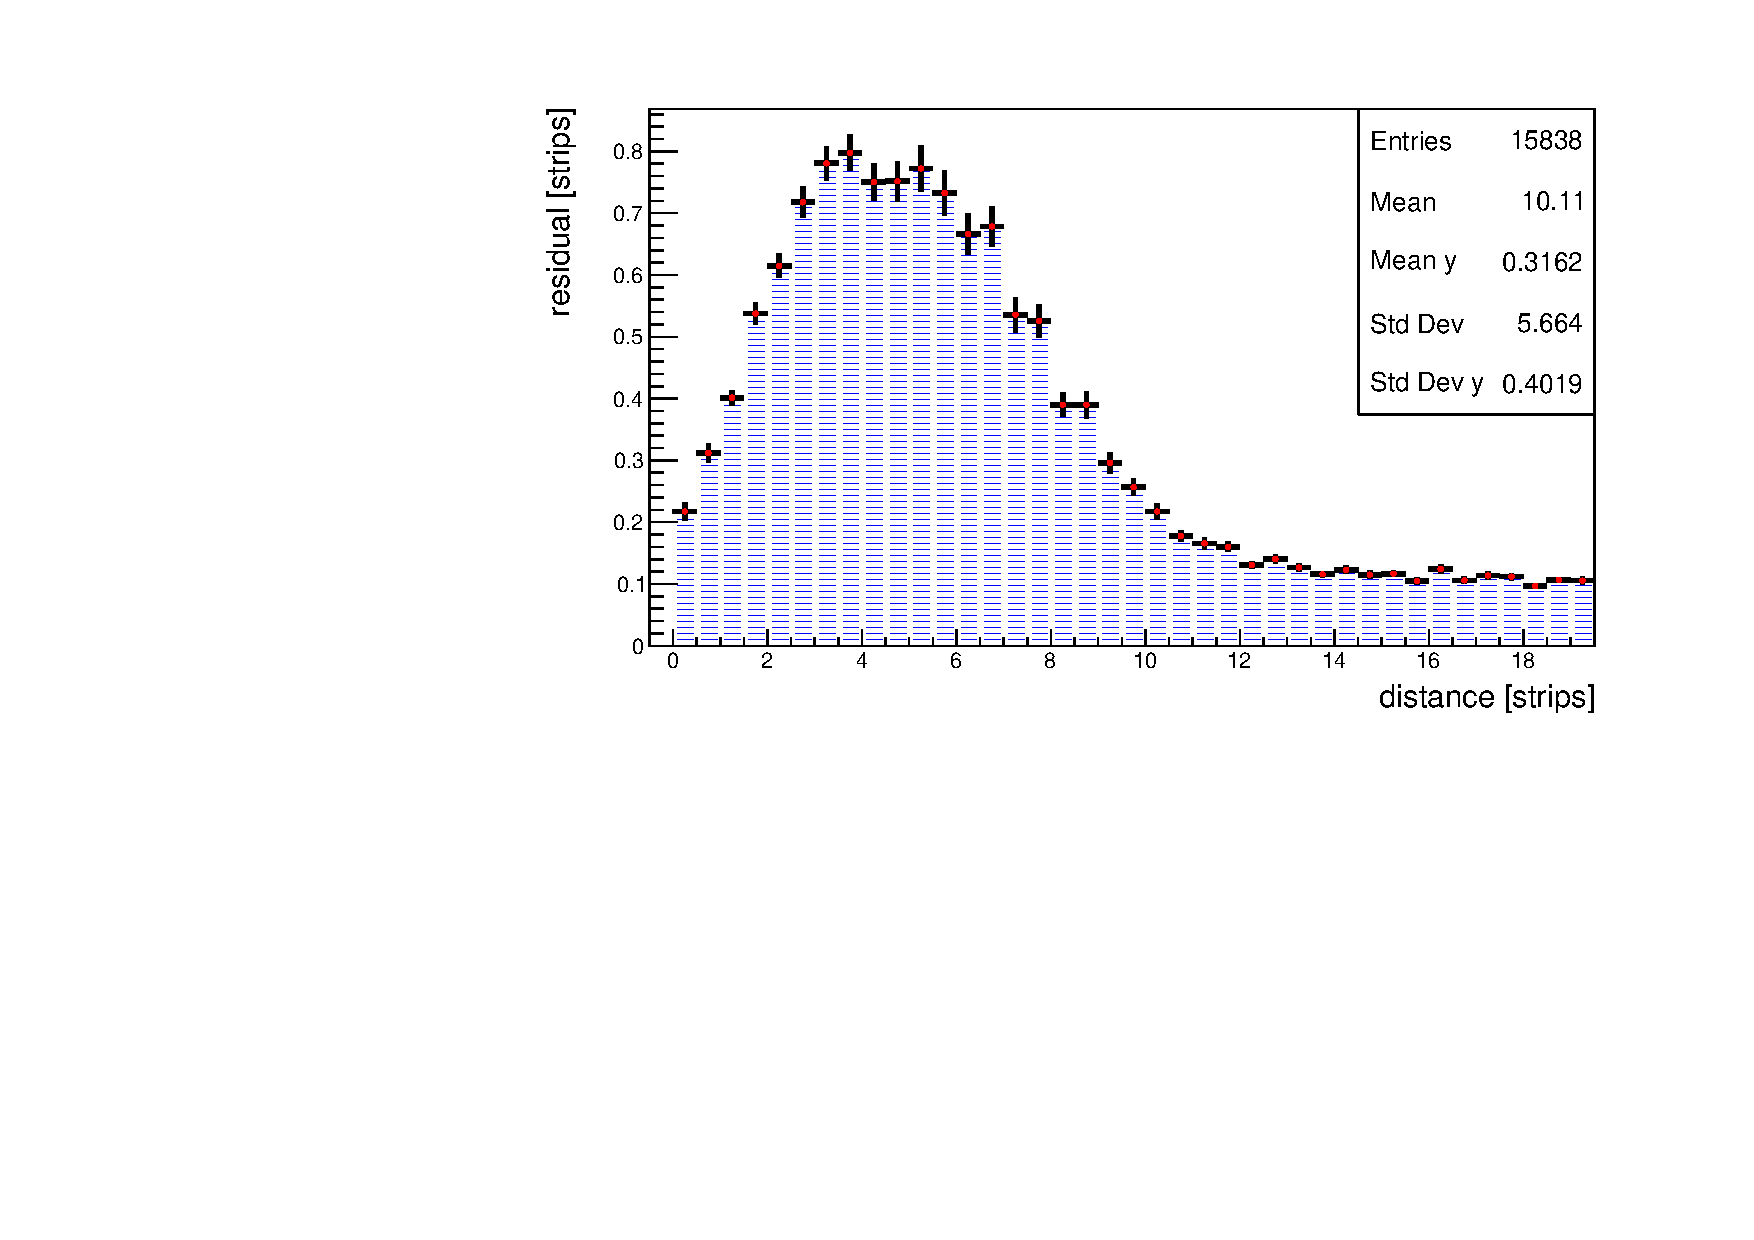
\includegraphics[width=\textwidth]{\pdirfive/res.pdf}
  \caption[Hit resolution as function of the two cluster distance]{Hit resolution of two separate clusters in a same plane as function of the distance between the two. The unit are given in strips size, where a single strip has a size of 256 $\mu$m for the Micromegas used in the NA64 experiment.}
  \label{fig:res-hit}
\end{figure}

\subsection{WCAL optimization}
\label{ch5:sec:new-vismode-setup-wcal}

The most important change in design to boost the signal yield is the increase of the probability of decay outside the target-dump for the $\DMX$. We see from Eq.\ref{eqn:length} that this number scales linearly on both the nominal energy of the beam the dimension of the dump. In 2018, the energy was already increased to 150 \gev to boost this probability. Additional increase in energy will have several demerit, amounting to a larger background in the sample due to the production mechanism of the beam and a shorter bending that would reduce the rejection power of the SRD. Instead, a new design of the WCAL with short longitudinal dimension can achieve the same purpose while keeping the background under check.

To design the new calorimeter structure, the figure of merit is the signal efficiency, which is defined mostly by the number of $\DM$ that decay outside the WCAL. This was quantified by a detailed MC-simulation of the setup used to generate the energy spectrum and the decay kinematics of the $\DM$.

%%% radiation length of tungsten collected at http://pdg.lbl.gov/2014/AtomicNuclearProperties/HTML/tungsten_W.html
In the design used in previous searches, the WCAL had 34 layers in total, each of them consisting of a converter layer made of 3 mm of tungsten and an active part made of a 2 mm plastic scintillators. This sums to a total of $\sim$30X$_0$. Reducing the dimension of the WCAL would impact the radiation length used to contain the main shower and hence change the background conditions. To avoid this, the new design of the calorimeter was studied under the principle that the optimal radiation length should be approximately 30X$_0$. The three following design were considered:

\begin{itemize}
\item An initial part of 9 layers using the original layer structure followed by an additional 25 layers of only tungsten.
\item A calorimeter consisting of 17 layers with layer-structure: 6mm tungsten + 2mm plastic scintillator.
\item A calorimeter consisting of 12 layers with a different structure: 9mm tungsten + 2mm plastic scintillator.
\end{itemize}

In all designs, the initial 5 layers forming the pre-shower part are still used for efficient hadron rejection. Despite its longer length, the first design grants a good energy resolution and a good hermeticity. In the second and third case, the calorimeter is more compact but has a worse energy resolution due to the thicker converter. A sketch of the two last designs is shown in Fig.\ref{fig:wcal-design} and compared to the original one used in the previous searches.

The third design was chosen to be the most suited for our search. The loss in energy resolution has almost no impact on the signal efficiency. The reason is that the short lifetime of the $\DM$ favors the detection of the ones produced at high energy that are able to escape the dump more efficiently. These $\DM$ carry most of the initial e$^-$ energy outside of the WCAL in the calorimeter placed downstream (ECAL). Hence, the energy is reconstructed with a precision of $<$1\% regardless of the WCAL structure. The second and third designs are compared to the original WCAL in Table \ref{tab:wcal-length-results}.

\begin{center}
\begin{table}[tbh!]
\begin{tabular}{lcr}
  WCAL structure [mm](layers)  & $\epsilon$  & EOT to cover $\DM$ at 90\% confidence [$10^{10}$] \\
  \hline
  ECAL1:3+2(34)                & 0.001   & 17$\pm$3.4                                            \\ 
  ECAL1:6+2(17)                & 0.001   & 7$\pm$0.9                                             \\
  ECAL1:9+2(12)                & 0.001   & 6$\pm$0.7                                             \\
  ECAL1:3+2(34)                & 0.0012  & 85$\pm$4.7                                            \\
  ECAL1:6+2(17)                & 0.0012  & 24$\pm$6.9                                            \\  
  ECAL1:9+2(12)                & 0.0012  & 19$\pm$5                                              \\  
  \hline
\end{tabular}
\caption[Possible WCAL design and with their possible experimental reach]{Number EOT required to cover $\DM$ at 90\% confidence using different WCAL designs in the visible mode setup proposed for 2021. The first entry describes the structure using the convention:
  ECALconverter-depth+counter-depth(number-of-layers).}
\label{tab:wcal-length-results}
\end{table}
\end{center}

\begin{figure}[tbh!]
  \centering
  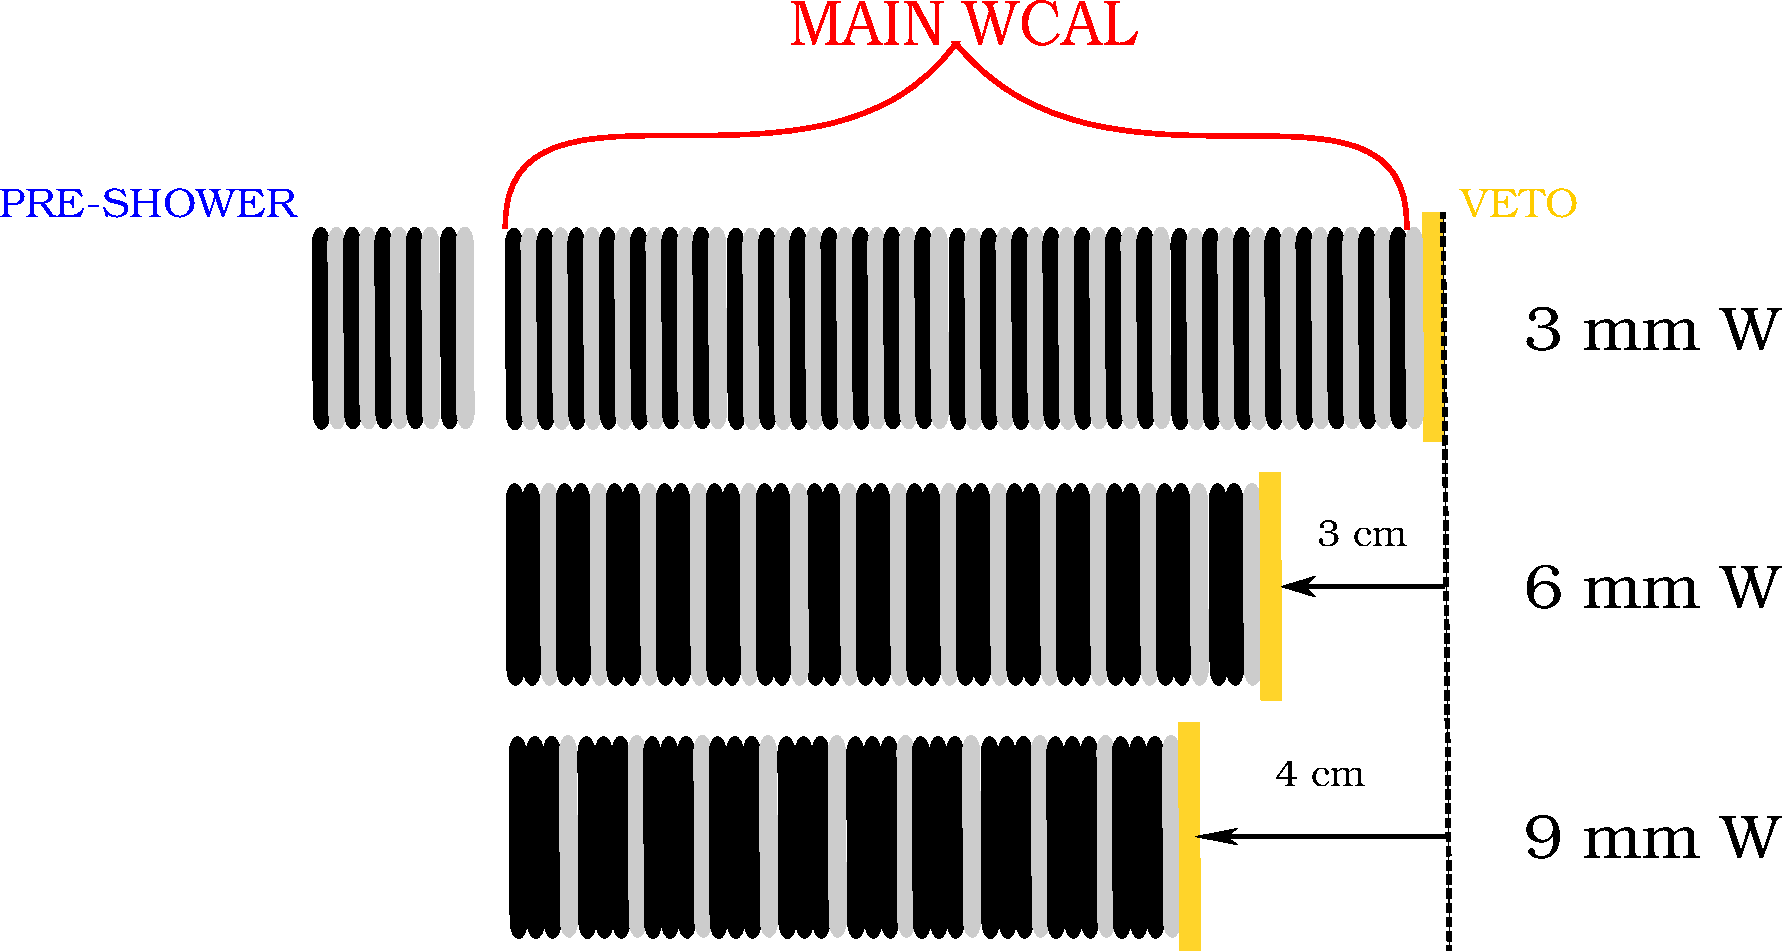
\includegraphics[scale=0.5]{\pdirfive/WCAL_design.pdf}
  \caption[New WCAL design for 2021]{Possible designs of the WCAL re-arranging the available tiles of 3 mm of Tungsten (W) and 2 mm of scintillator material. All designs posses the same radiation length of 30$X_0$.}
  \label{fig:wcal-design}
\end{figure}


\subsubsection{Background and sensitivity}
\label{ch5:sec:background-sensitivity}

A preliminary study of background was performed in this novel setup. As discussed in Sec.\ref{ch3:sec:bkg} the main source of background is coming from the production of $\ks$ in the WCAL escaping the dump and decaying in the vacuum tube as the $\DM$. The decay products can potentially mimic the signal either in the chain K$^0_S \rightarrow \pi^0 \pi^0$ where $\ee$ pair are produced in the $\gamma$ conversion of the photon pair into an $\ee$ or in the rare decays $\pi^0 \rightarrow \gamma e^- e^+$. To estimate the impact of such background a simulation of 5$\times 10^6$ $\ks$ was performed using the energy spectrum expected from the production of this particle via electro-nuclear interactions.
The conservative assumption of the simulation is that the $K^0_S$ is produced in an inelastic scattering in the WCAL where all the energy is deposited inside the dump without leaving a significant signature in W2. It was found that only 3\% of the events left a shower separation in the ECAL similar to the one expected from $\DM$. Less than 1\% of the events are within the acceptance of the trackers. In the majority ($>$90\%) of the surviving events the $\ks$ has an energy $<$60 \gev. This spectrum is significantly different from the one predicted for the $\DM$, where 95\% of the spectrum is above 100 \gev with a sharp peak at 150 \gev (the nominal beam energy). Finally, no event in the sample was reconstructed with an invariant mass compatible with the $\DM$, the closest one being reconstructed at 280 MeV. This is well above any $A'$ scenario in the reach of the NA64 experiment \cite{Banerjee:2019hmi}. As the new WCAL design conserves the hermeticity of 30$X_0$, the background coming from $\gamma$-punchtrough (see Sec.\ref{ch3:sec:bkg}) is not expected to increase in the new setup. This contribution is hard to study in detail using MC simulation, it was however demonstrated in our previous measurements \cite{Banerjee:2019hmi} that longer setup adds a suppression to this background which is therefore expected to decrease due to the longer decay volume. As both neutral-punchtrough and $\ks$ are not expected to increase, one can conservatively put the background at a level of $0.01<$ (see Table \ref{tab:vis-bkg}).

An analysis based on the simulated data was conducted to estimate the reach of the experiment using the proposed setup. Most of the selection criteria already applied in our previous searches were used for this study. Additionally, a good separation of at least 8 cm is required between the two electromagnetic showers and the reconstructed invariant mass is selected to be within 10\% of the expected $\DM$ mass. The expected signal yield was computed after all the cuts were applied and used to calculate the 90\% exclusion of different $\DM$ scenarios. The results of the computation are presented in Fig.\ref{fig:exclusion-x17} that shows the number of EOT necessary to probe a specific $\DM$ scenario. Assuming a trigger-rate similar to the one observed during 2018 visible-mode data taking, a projection of the days needed is also shown. As expected, the EOTs required to probe a specific $\DM$ model increases exponentially with the coupling strength $\epsilon$, since the signal yield is dominated by the probability of $\DM$ to exit the dump. The conclusion is that the complete range $\epsilon < 1.4 \times 10^{-3}$ of $\DM$ parameter space proposed in \cite{PhysRevD.95.035017} can be covered in approximately 3 months of beam time by accumulating $\sim 7 \times 10^{11}$ EOTs. Models with V$\pm$A coupling mentioned in Sec.\ref{ch1:sec:dm-candidates} on the other hand can be covered faster ($<$10 days) due to the smaller allowed coupling. 

\begin{figure}[htb!]
  \centering
  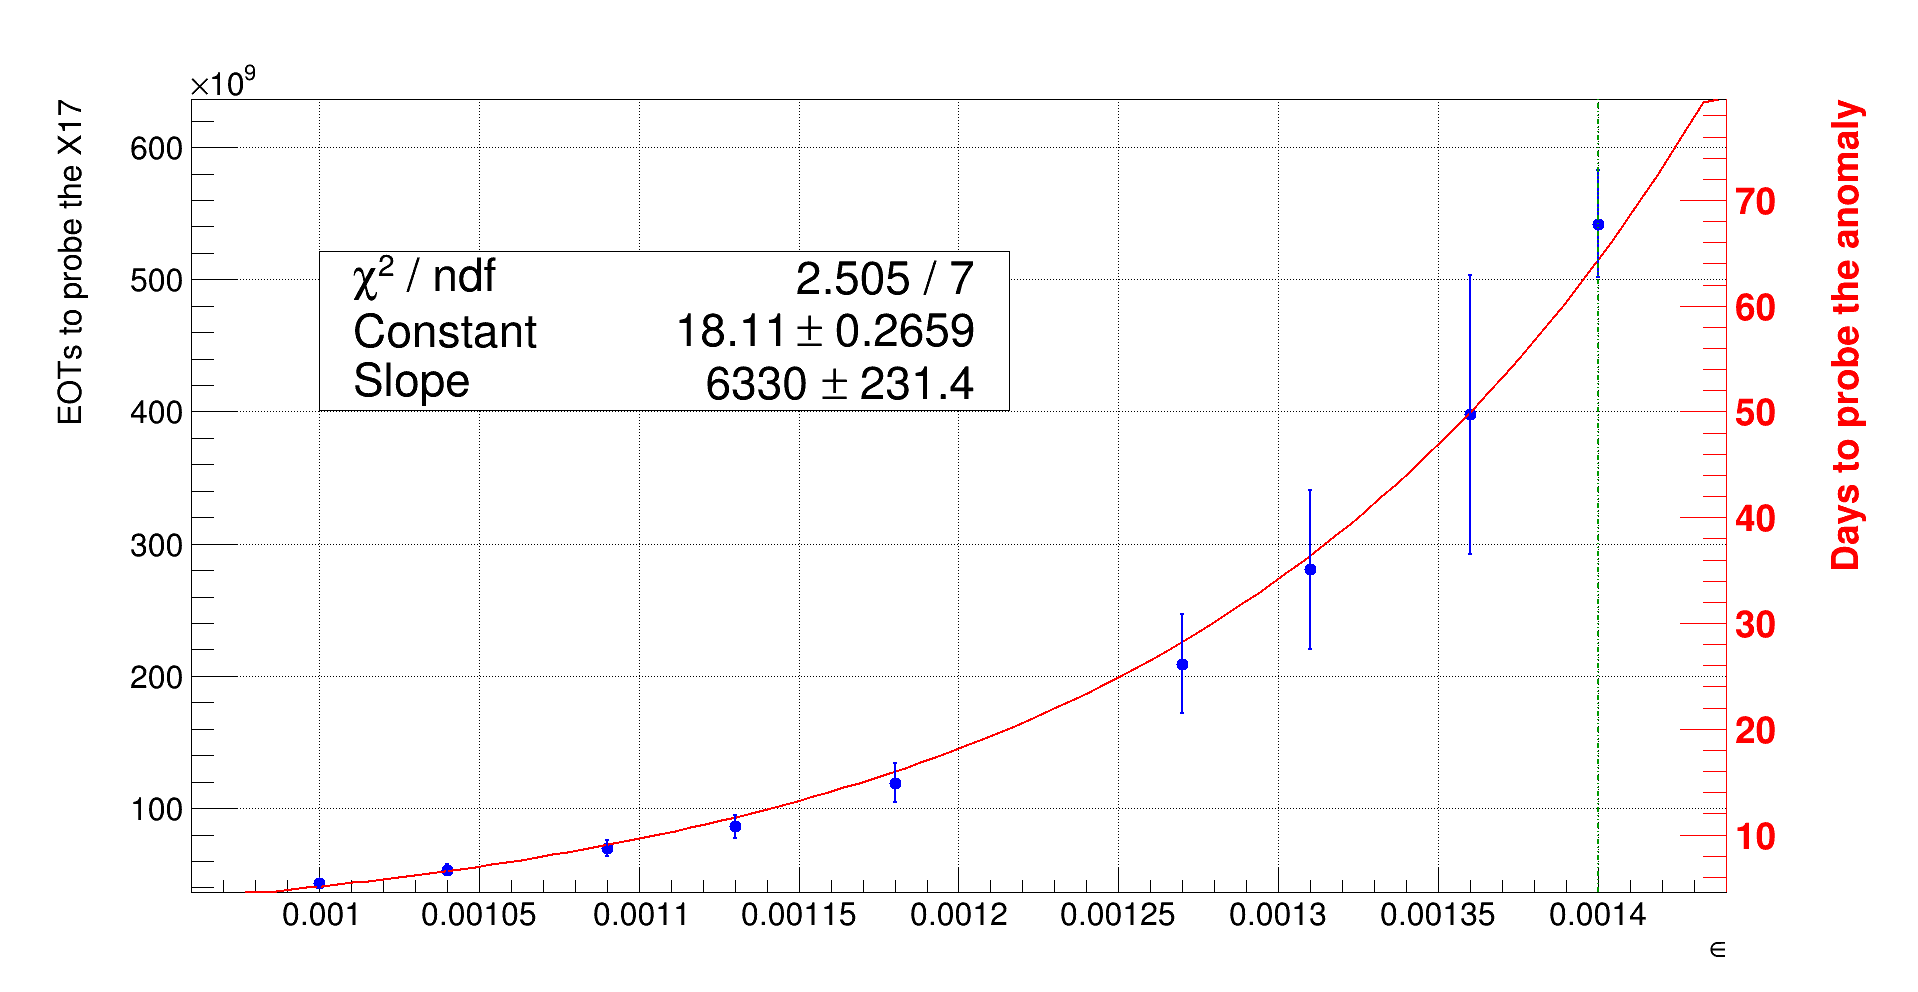
\includegraphics[width=\textwidth]{\pdirfive/exclusion_167_exclusion.png}
  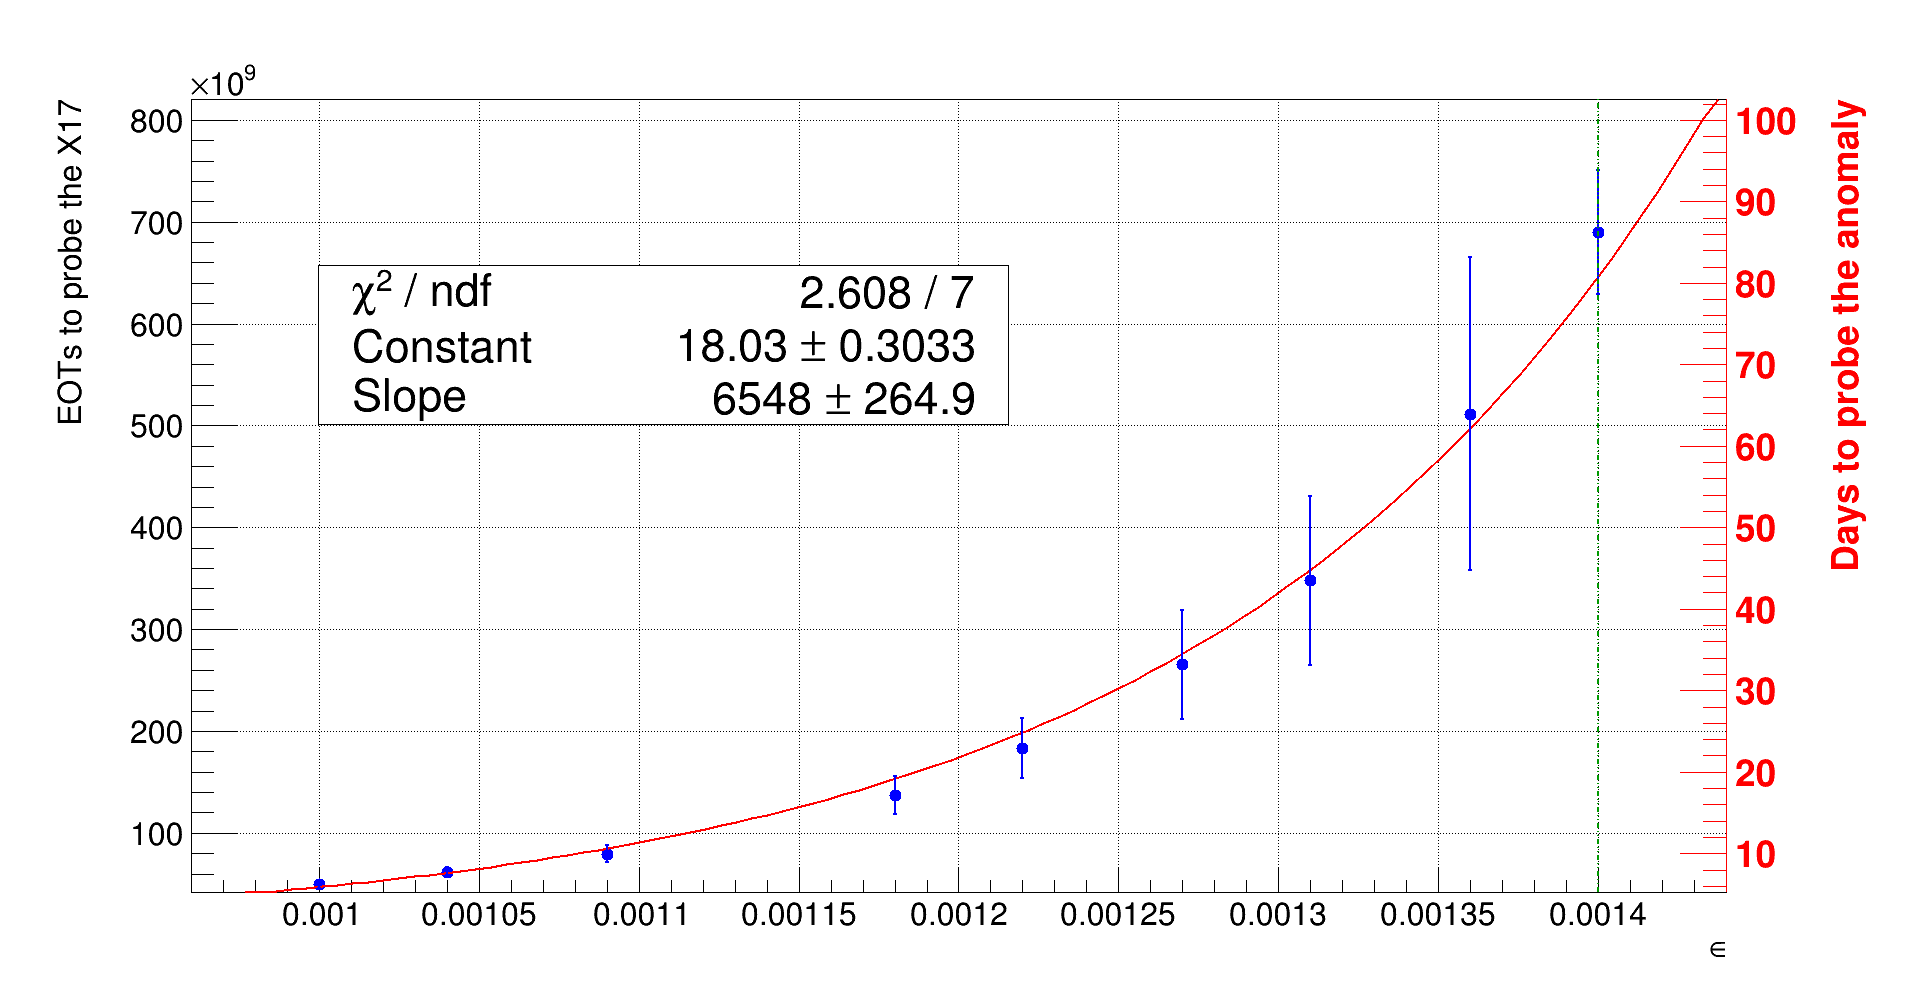
\includegraphics[width=\textwidth]{\pdirfive/exclusion_170_exclusion.png}
  \caption[EOT to X17 exclusion]{Number of EOTs needed to probe the $\DM$ with an exclusion limit of 90\% assuming negligible background as function of $\epsilon$ on the left y-axis, while the number of days required to accumulate the correspondent number of EOTs is shown in the right y-axis and is based on the trigger-rate measured during the 2018 visible mode data taking \cite{Banerjee:2019hmi}. A green dashed line shows the maximum $\epsilon$ permitted if $\DM$ is interpreted as protophobic gauge boson \cite{PhysRevD.95.035017}. The detection efficiency for high $\epsilon$ is dominated by the probability of $\DM$ to exit the dump as it is shown by the exponential fit (red line). The plot is shown for the two most relevant mass scenarios suggested by the two experiments conducted by the ATOMKI group, i.e. 16.7 MeV (top) and 17.0 MeV (bottom) \cite{Krasznahorkay:2015iga,Krasznahorkay:2019lyl}.}
  \label{fig:exclusion-x17}
\end{figure}
  
\section{A new approach: Muon mode setup}
\label{ch5:sec:muon-mode-setup}

%%% Local Variables:
%%% mode: latex
%%% TeX-master: "../PhDthesis"
%%% End:
